% !TeX root = ../thesis.tex
\chapter{Appendices to Chapter~\ref{ch:permapprox}}
\label{sec:app:permApprox}

% t-test: shape estimates
\begin{figure}[H]
  \centering
  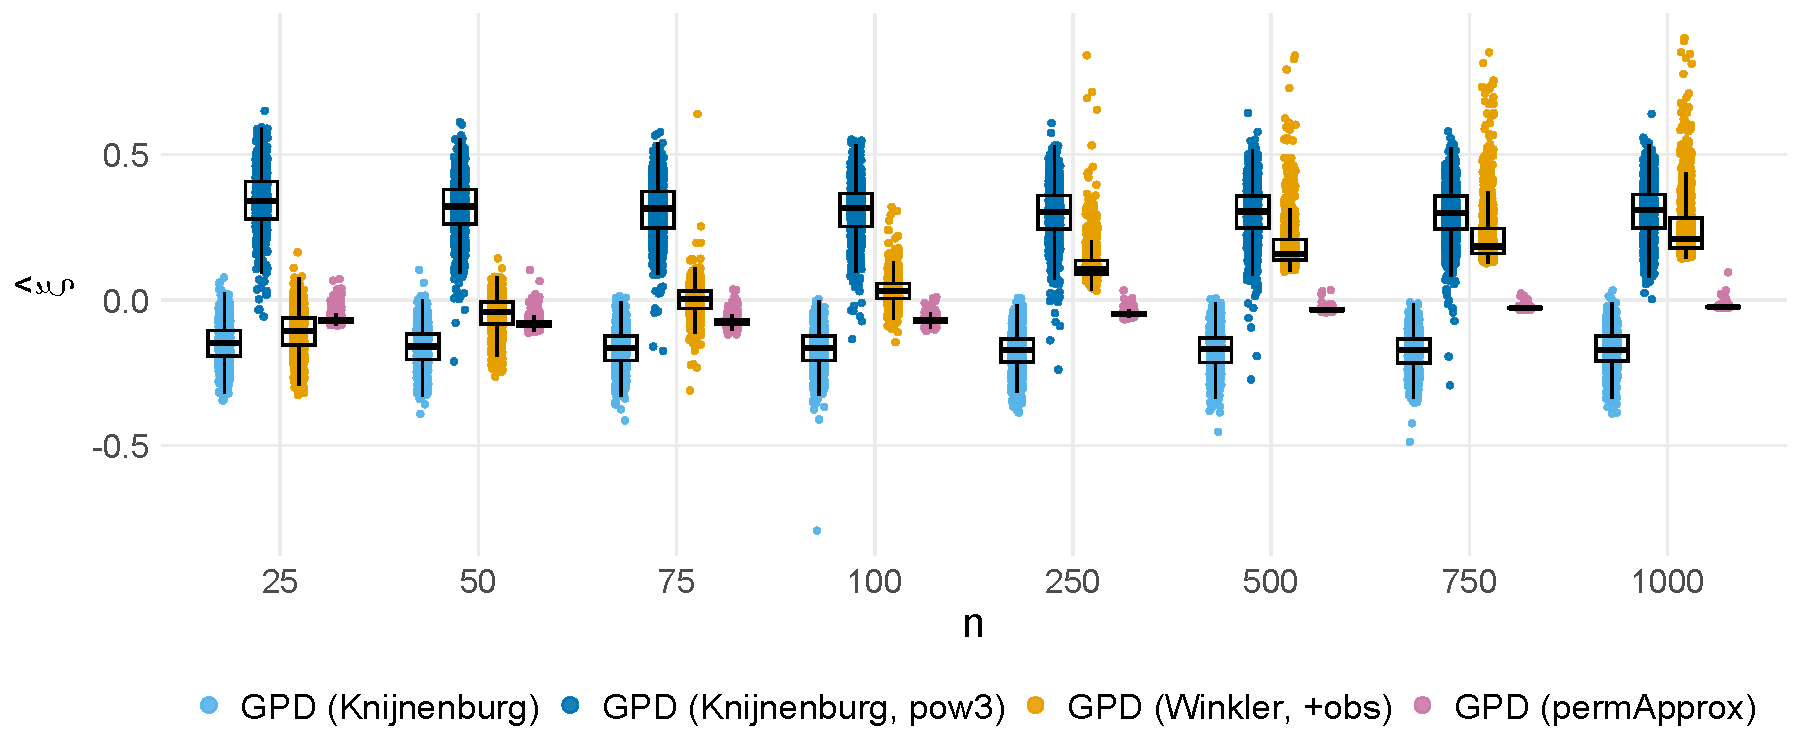
\includegraphics[width=\textwidth]{../ch06_permapprox/simulations/perm_ttest/figures/05_p_approx_methods/sim_ttest_papprox_shape_estimates_by_n-1.pdf}
  \caption{\textbf{Two-sample t-test with Gaussian data:} Estimated GPD shape values across sample sizes for the compared GPD-based methods. Effect size and number of permutations are fixed to $d=1$ and $B=1000$, respectively. Points indicate individual replicates (1000 per setting).}
  \label{fig:app:6perm:ttest_shapes_by_n}
\end{figure}

% t-test: p-values by n
\begin{figure}[ht]
  \centering
  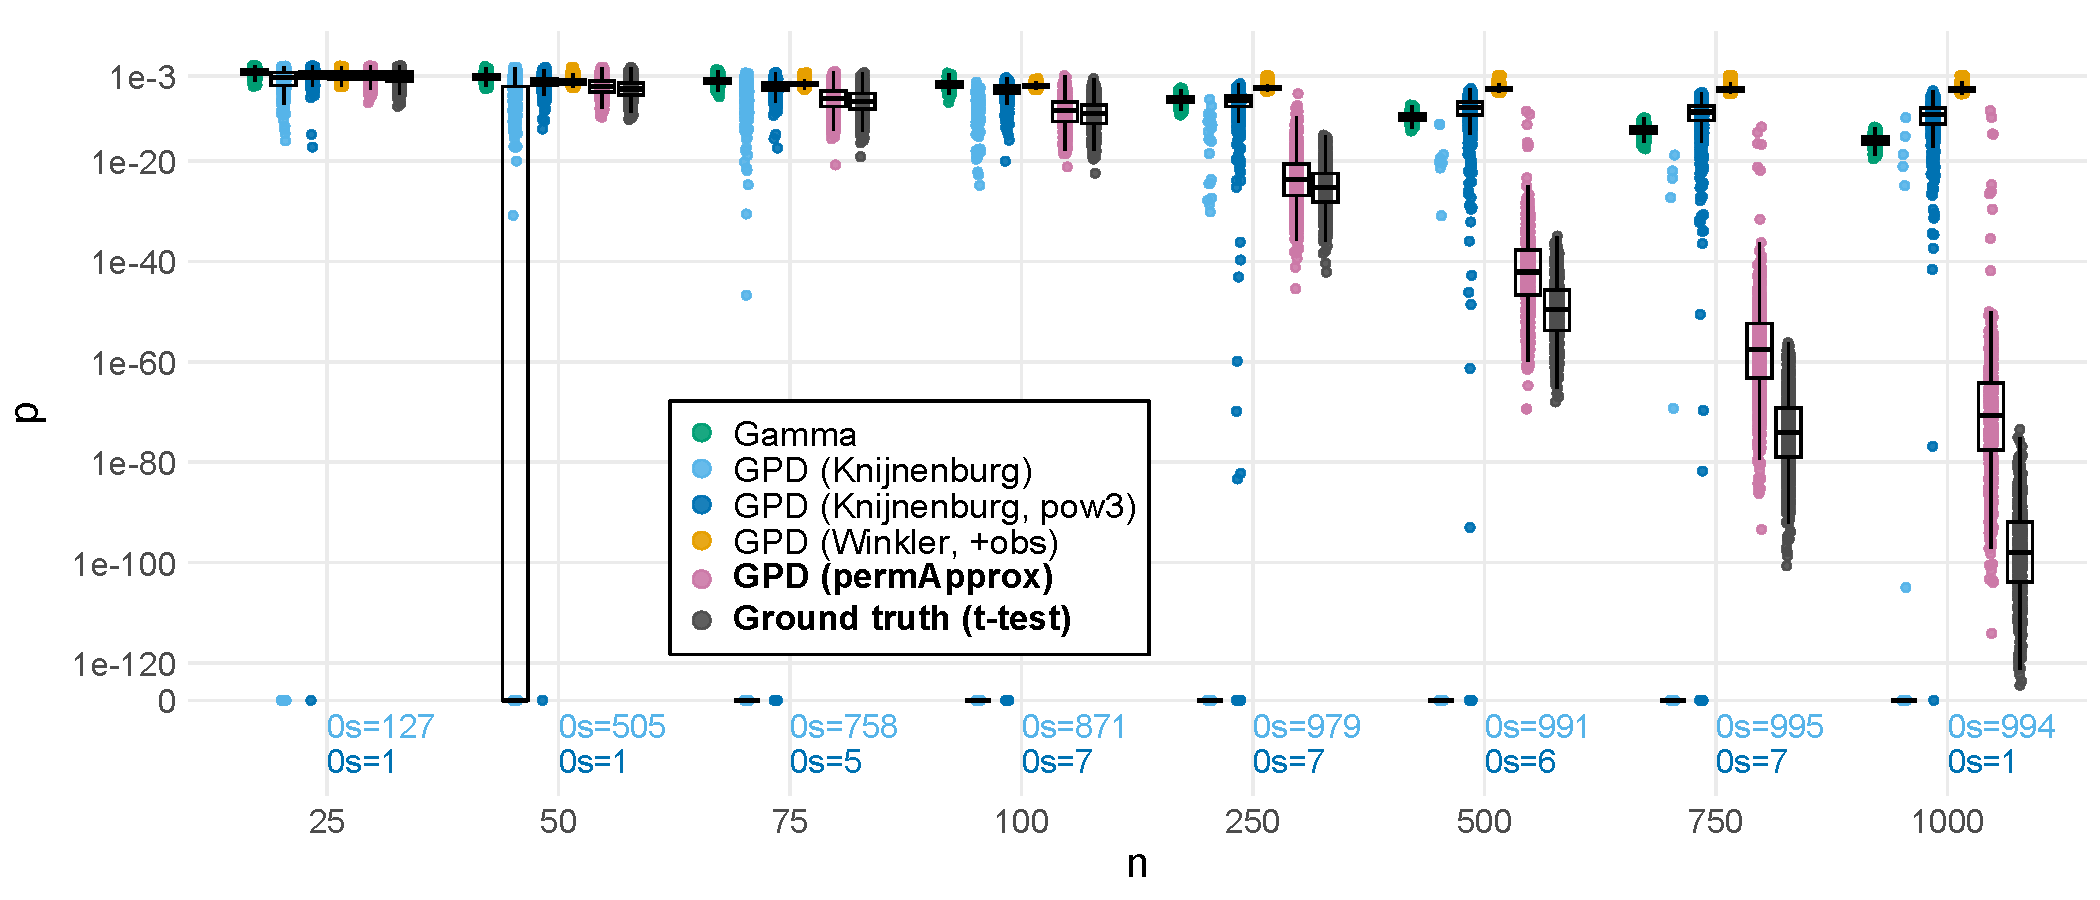
\includegraphics[width=\textwidth]{../ch06_permapprox/simulations/perm_ttest/figures/05_p_approx_methods/sim_ttest_papprox_pvals_by_n-1.pdf}
  \caption{\textbf{Two-sample t-test with Gaussian data:} $p$-values produced with the different approximation methods, in comparison to Student's \textit{t}-test $p$-values across varying sample sizes.
  Effect size and number of permutations are fixed to $d=1$ and $B=1000$, respectively. Points indicate individual replicates (1000 per setting). 
  Counts of exact zeros are shown below each group as ``\texttt{0s}=x'' in the corresponding color.
  Zero $p$-values are mapped to a small constant floor so they appear at ``0'' on the $y$-axis. The y-axis is on a log10 scale, while tick labels show the original $p$-values.}
  \label{fig:app:6perm:ttest_pvals_by_n}
\end{figure}

% t-test: p-values by d and B
\begin{figure}[H]
  \centering
  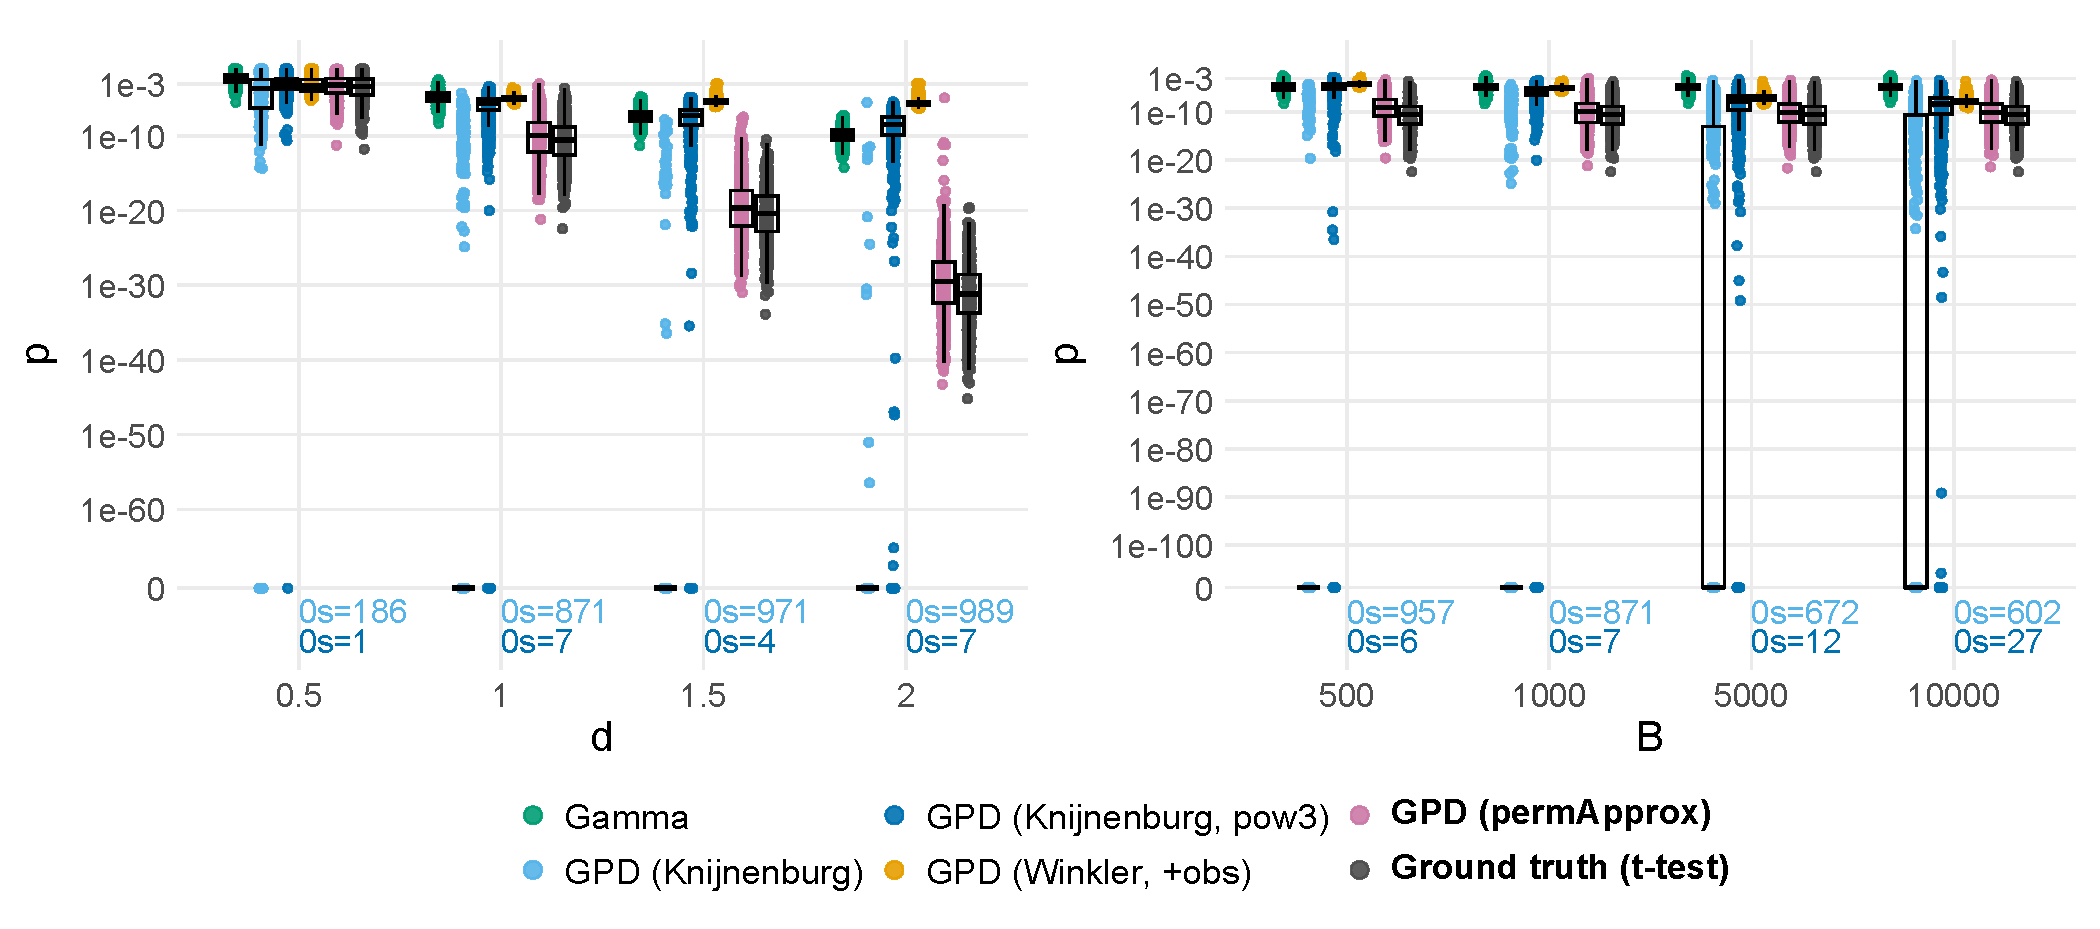
\includegraphics[width=\textwidth]{../ch06_permapprox/simulations/perm_ttest/figures/05_p_approx_methods/sim_ttest_papprox_pvals_by_d_and_B-1.pdf}
  \caption{\textbf{Two-sample t-test with Gaussian data:} Approximated permutation $p$-values, stratified by effect size $d$ (left panel) and number of permutations $B$ (right panel). Fixed values (if not stratified): $n=100$, $d=1$ and $B=1000$. Points indicate individual replicates (1000 per setting). 
  Counts of exact zeros are shown below each group as ``\texttt{0s}=x'' in the corresponding color.
  For plotting only, zero $p$-values are mapped to a small constant floor so they appear at ``0'' on the $y$-axis. The y-axis is on a log10 scale, while tick labels show the original $p$-values.}
  \label{fig:app:6perm:ttest_pvals_by_d_and_B}
\end{figure}

% t-test: ratios by d and B
\begin{figure}[H]
  \centering
  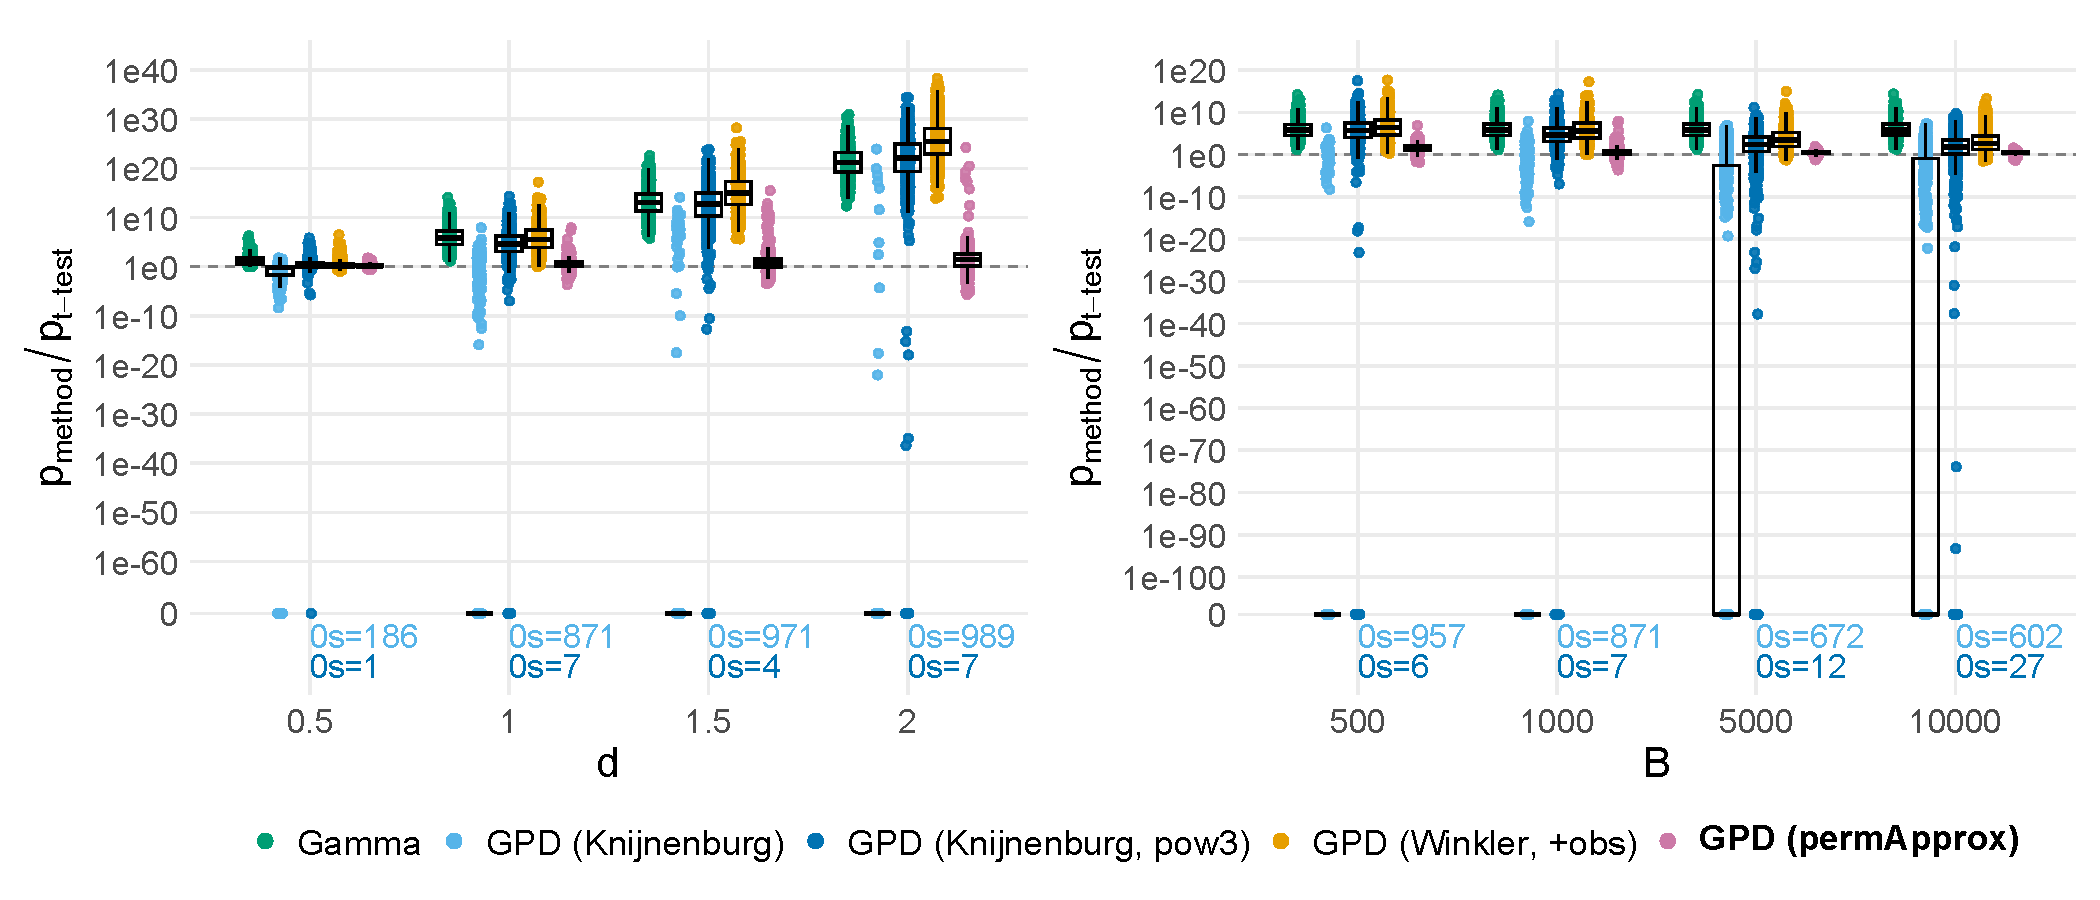
\includegraphics[width=\textwidth]{../ch06_permapprox/simulations/perm_ttest/figures/05_p_approx_methods/sim_ttest_papprox_ratios_by_d_and_B-1.pdf}
  \caption{\textbf{Two-sample t-test with Gaussian data:} Ratios of approximated to ground-truth $p$-values: $p_{\text{method}} / p_{t\text{-test}}$, stratified by effect size $d$ (left panel) and number of permutations $B$ (right panel). Fixed values (if not stratified): $n=100$, $d=1$ and $B=1000$. Points indicate individual replicates (1000 per setting). 
  Counts of exact zeros are shown below each group as ``\texttt{0s}=x'' in the corresponding color.
  For plotting only, zero $p$-values are mapped to a small constant floor so they appear at ``0'' on the $y$-axis ratios.}
  \label{fig:app:6perm:ttest_ratios_by_d_and_B}
\end{figure}

% Wilcoxon: p-values by n
\begin{figure}[H]
  \centering
  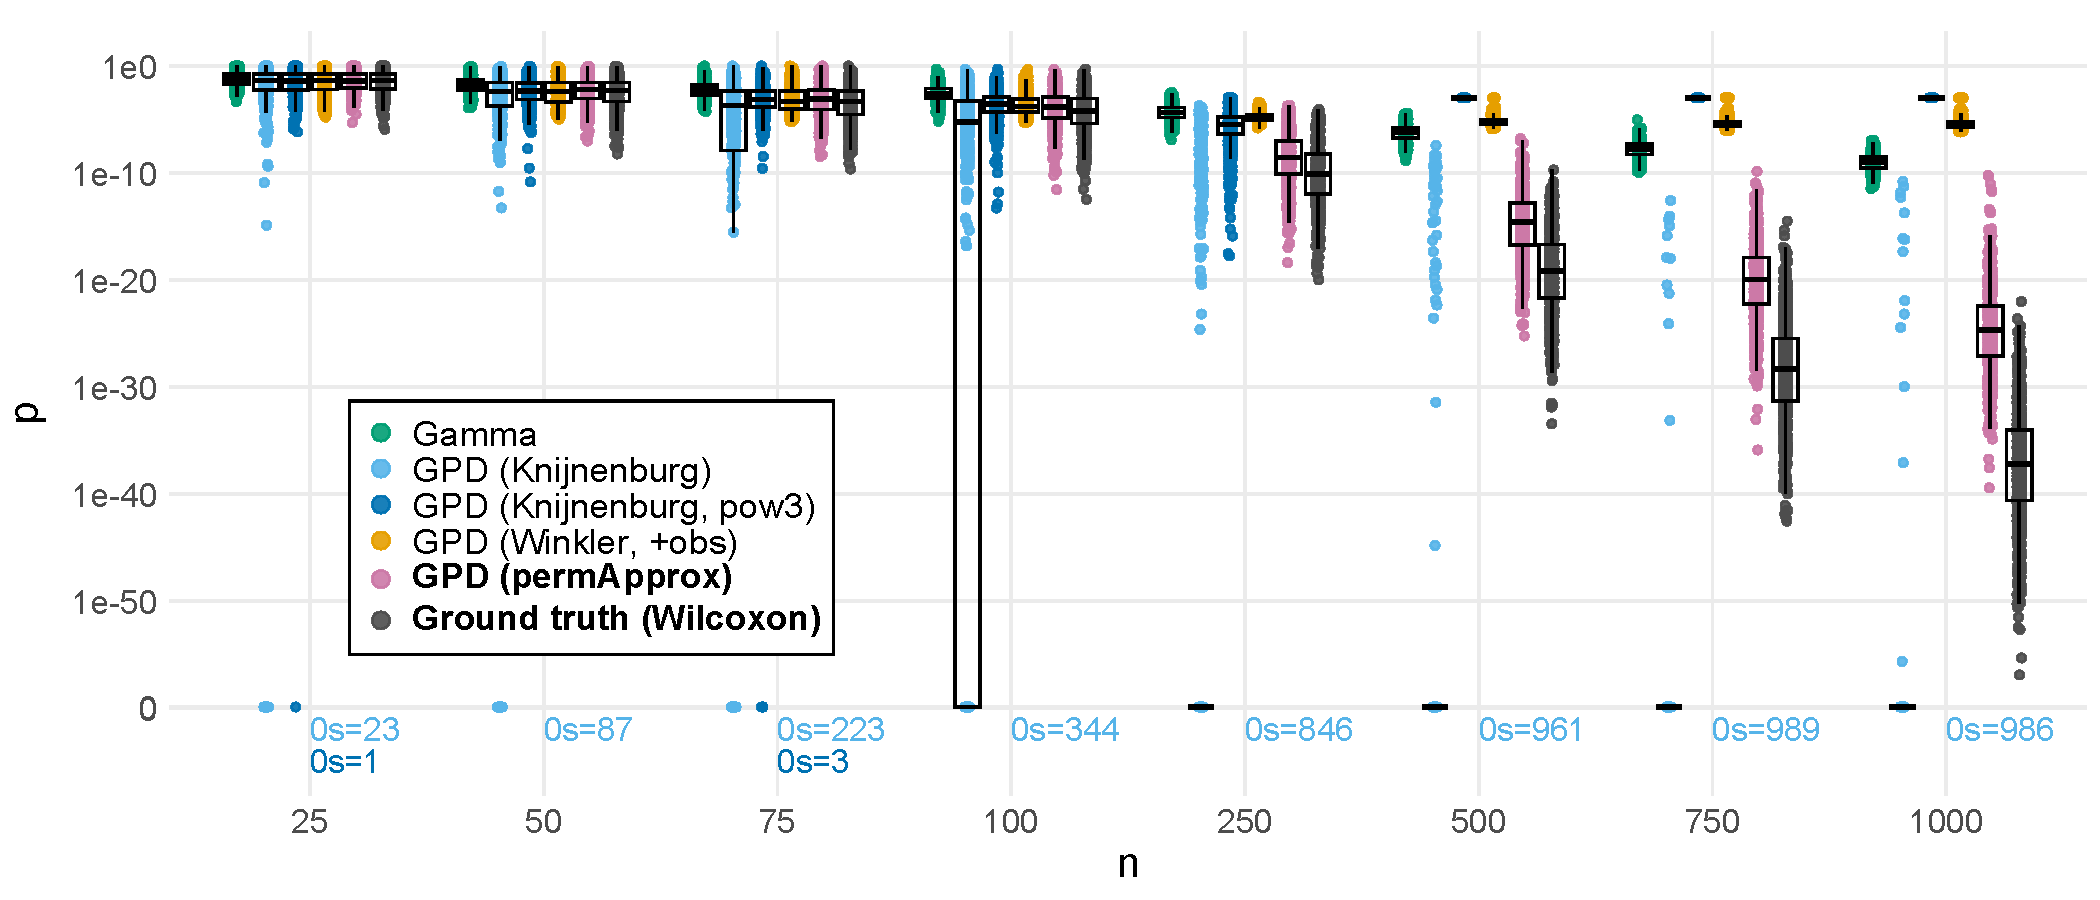
\includegraphics[width=\textwidth]{../ch06_permapprox/simulations/perm_wilcox/figures/02_p_approx_methods/sim_wilcox_papprox_pvals_by_n-1.pdf}
    \caption{\textbf{Wilcoxon rank-sum test with exponential data:} Approximated permutation $p$-values, stratified by sample size $n$. Fixed values: $d=1$ and $B=1000$. Points indicate individual replicates (1000 per setting). 
    Counts of exact zeros are shown below each group as ``\texttt{0s}=x'' in the corresponding color. 
    For plotting only, zero $p$-values are mapped to a small constant floor so they appear at ``0'' on the $y$-axis. The y-axis is on a log10 scale, while tick labels show the original $p$-values.}
  \label{fig:app:6perm:wilcox_pvals_by_n}
\end{figure}

% Wilcoxon: p-values by d and B
\begin{figure}[H]
  \centering
  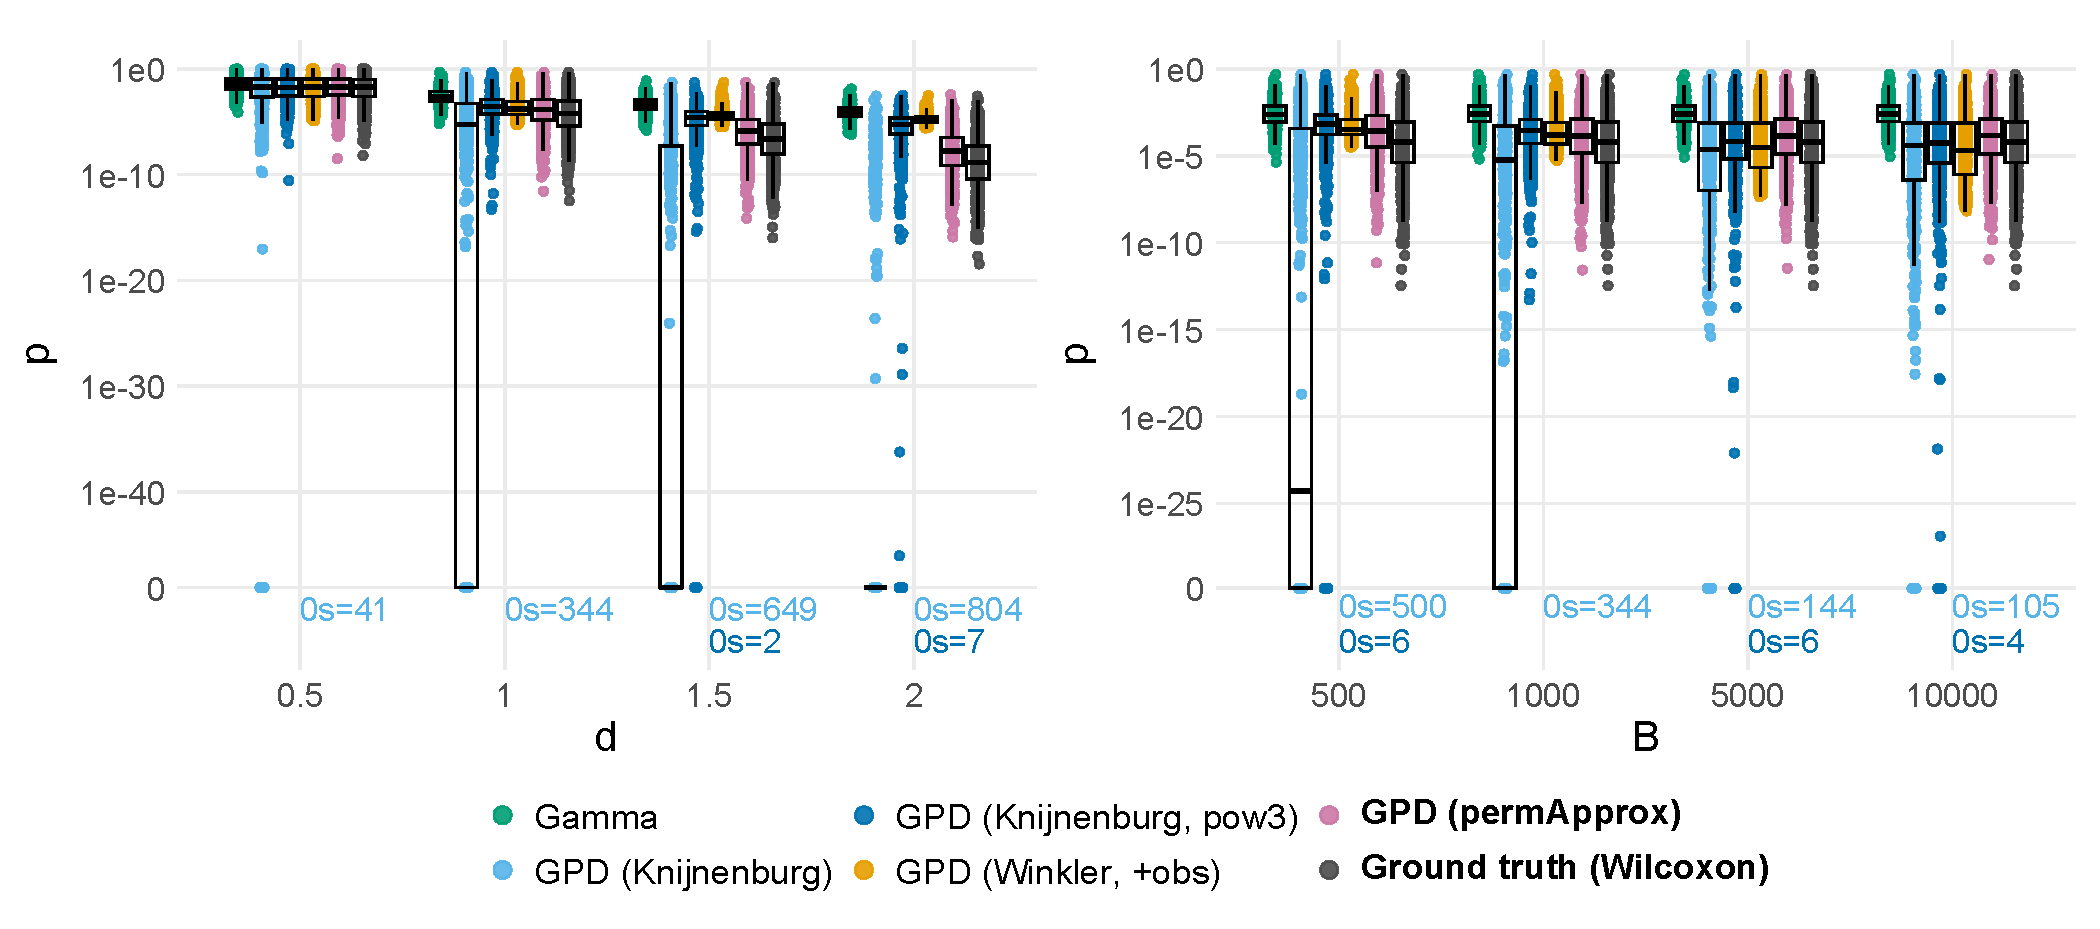
\includegraphics[width=\textwidth]{../ch06_permapprox/simulations/perm_wilcox/figures/02_p_approx_methods/sim_wilcox_papprox_pvals_by_d_and_B-1.pdf}
  \caption{\textbf{Wilcoxon rank-sum test with exponential data:} Approximated permutation $p$-values, stratified by effect size $d$ (left panel) and number of permutations $B$ (right panel). Fixed values (if not stratified): $n=100$, $d=1$ and $B=1000$. Points indicate individual replicates (1000 per setting). 
  Counts of exact zeros are shown below each group as ``\texttt{0s}=x'' in the corresponding color.
  For plotting only, zero $p$-values are mapped to a small constant floor so they appear at ``0'' on the $y$-axis. The y-axis is on a log10 scale, while tick labels show the original $p$-values.}
  \label{fig:app:6perm:wilcox_pvals_by_d_and_B}
\end{figure}

% Wilcoxon: ratios by d and B
\begin{figure}[H]
  \centering
  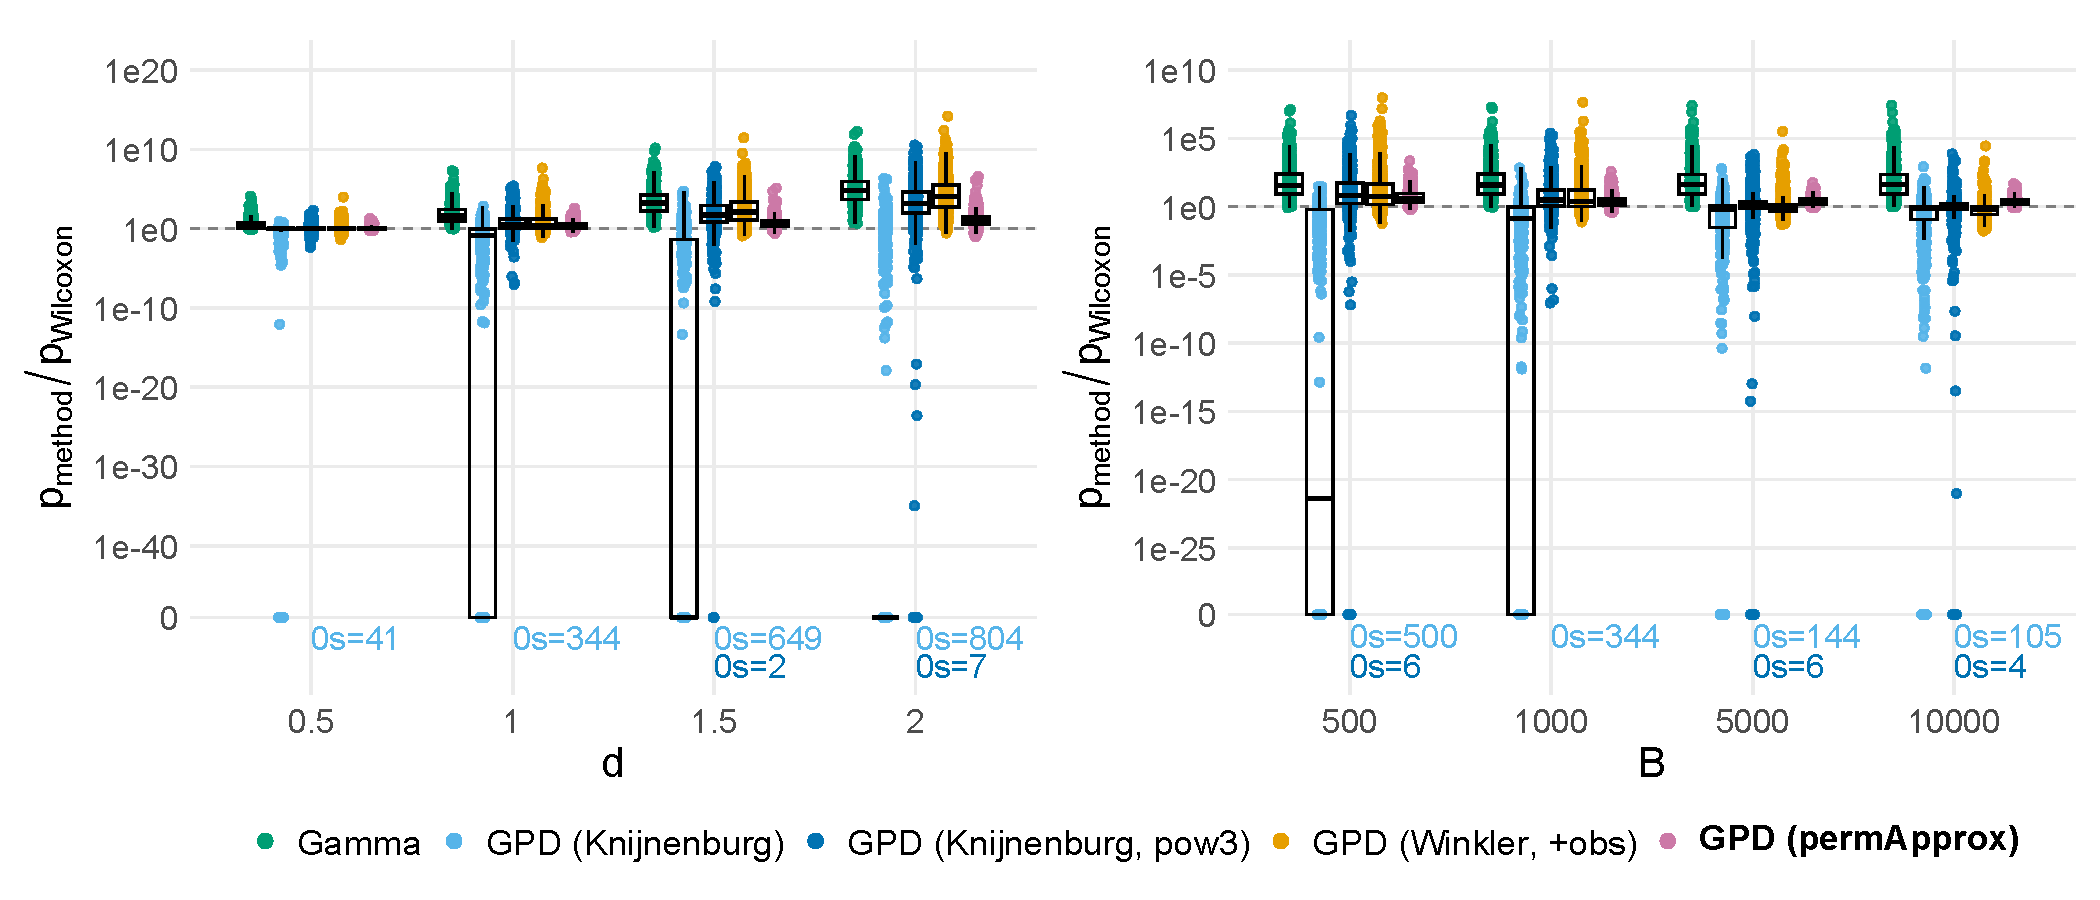
\includegraphics[width=\textwidth]{../ch06_permapprox/simulations/perm_wilcox/figures/02_p_approx_methods/sim_wilcox_papprox_ratios_by_d_and_B-1.pdf}
  \caption{\textbf{Wilcoxon rank-sum test with exponential data:} Ratios of approximated to ground-truth $p$-values: $p_{\text{Method}} / p_{\text{Wilcoxon}}$, stratified by effect size $d$ (left panel) and number of permutations $B$ (right panel). Fixed values (if not stratified): $n=100$, $d=1$ and $B=1000$. Points indicate individual replicates (1000 per setting). 
  Counts of exact zeros are shown below each group as ``\texttt{0s}=x'' in the corresponding color.
  For plotting only, zero $p$-values are mapped to a small constant floor so they appear at ``0'' on the $y$-axis. The y-axis is on a log10 scale, while tick labels show the original ratios.}
  \label{fig:app:6perm:wilcox_ratios_by_d_and_B}
\end{figure}
